\documentclass[10pt,twocolumn]{article}

\usepackage[margin=0.72in]{geometry}
\usepackage{amsmath}
\usepackage{amssymb}
\usepackage{booktabs}
\usepackage{graphicx}
\usepackage[hidelinks]{hyperref}
\usepackage{microtype}

\graphicspath{
  {Result_Test/step1_minimal_bright_dark/Eta_scan/Analysis/}
  {Result_Test/etape_2/Analysis/}
  {Result_Test/etape_3/Analysis/}
  {Result_Test/etape_4/Analysis/}
}

\title{\vspace{-1.2em}
Progress Report on a Minimal Bright--Dark Model for Nonlinear SOC Signatures in a Spin-Peierls Context}
\author{}
\date{\vspace{-1.5em}}

\begin{document}
\maketitle

\begin{abstract}
This note summarizes the modeling work completed so far for a minimal
bright--dark Liouville-space model motivated by nonlinear spectroscopy of
CuGeO$_3$-like spin chains.  The goal is not yet to provide a full microscopic
description of CuGeO$_3$, but to define and validate a sequence of numerical
controls capable of separating three possible origins of a nonlinear signal:
constant bright--dark spin-orbit mixing, lattice or spin-Peierls dimerisation,
and local spin-correlation effects.  The present results show that a scalar
renormalisation of bright--dark mixing is insufficient to distinguish
dimerisation from local spin correlations.  Adding an explicit dynamical
lattice coordinate breaks this degeneracy, and independent temperature/field
trends provide a practical diagnostic for identifying whether a spectral
feature tracks the spin-Peierls order parameter or persists in the uniform
chain regime.
\end{abstract}

\section{Motivation}

The original objective was to formulate a tractable model for extracting
two-dimensional nonlinear spectra of an $S=1/2$ spin-chain material such as
CuGeO$_3$.  At low temperature, the dominant material physics is expected to be
strongly tied to the spin-Peierls lattice instability rather than to a bare
spin-orbit coupling (SOC) alone.  The working question is therefore more
specific: can nonlinear spectroscopy, especially when exciting $d$-band
degrees of freedom, reveal a contribution associated with SOC-like
bright--dark mixing while avoiding a false assignment of lattice-driven
features to SOC?

The strategy has been to build a sequence of minimal controls.  Each control
adds only one conceptual ingredient, so that failure modes remain interpretable.
The tests were implemented with the Liouville-space solver using third-order
one-quantum pathways generated by the NQ protocol, with emphasis on rephasing
spectra and finite-window integrals around diagonal and cross peaks.

\section{Minimal orbital model}

The common orbital sector contains a ground state $|g\rangle$, a dark excited
state $|D\rangle$, and a bright excited state $|B\rangle$.  The unperturbed
Hamiltonian is
\begin{equation}
H_0 =
\Delta_D |D\rangle\langle D|
+ \Delta_B |B\rangle\langle B|,
\end{equation}
with the bright state carrying the optical dipole.  Bright--dark mixing is
introduced through
\begin{equation}
L_{BD}=|D\rangle\langle B|+|B\rangle\langle D|.
\end{equation}
The simplest model uses
\begin{equation}
H_{\mathrm{mix}} = V_{BD} L_{BD}.
\end{equation}
For the validated runs summarized below, the representative orbital energies
were $\Delta_D=0.90$ eV and $\Delta_B=1.00$ eV, with broadening parameter
$\eta=10^{-3}$ unless otherwise noted.

\section{Step 1: minimal bright--dark validation}

The first test established that the solver and the finite-window analysis can
detect bright--dark mixing in a controlled two-level excited-state model.  The
control parameter was a static mixing amplitude $V_0$, compared against a
$V_0=0$ baseline.  Rephasing spectra were generated for several values of the
linewidth parameter $\eta$ and frequency-grid size $N_\omega$.

The important outcome is qualitative rather than a claim of perfect numerical
convergence.  The cross-window response is sensitive to $V_0$, but the
extracted finite-window integrals also depend on $\eta$ and grid resolution,
especially when narrow lines are sampled on a coarse grid.  This means Step 1
is sufficient as a validation of the spectral machinery and pathway extraction,
but not as a final convergence study.

\begin{figure}[t]
\centering
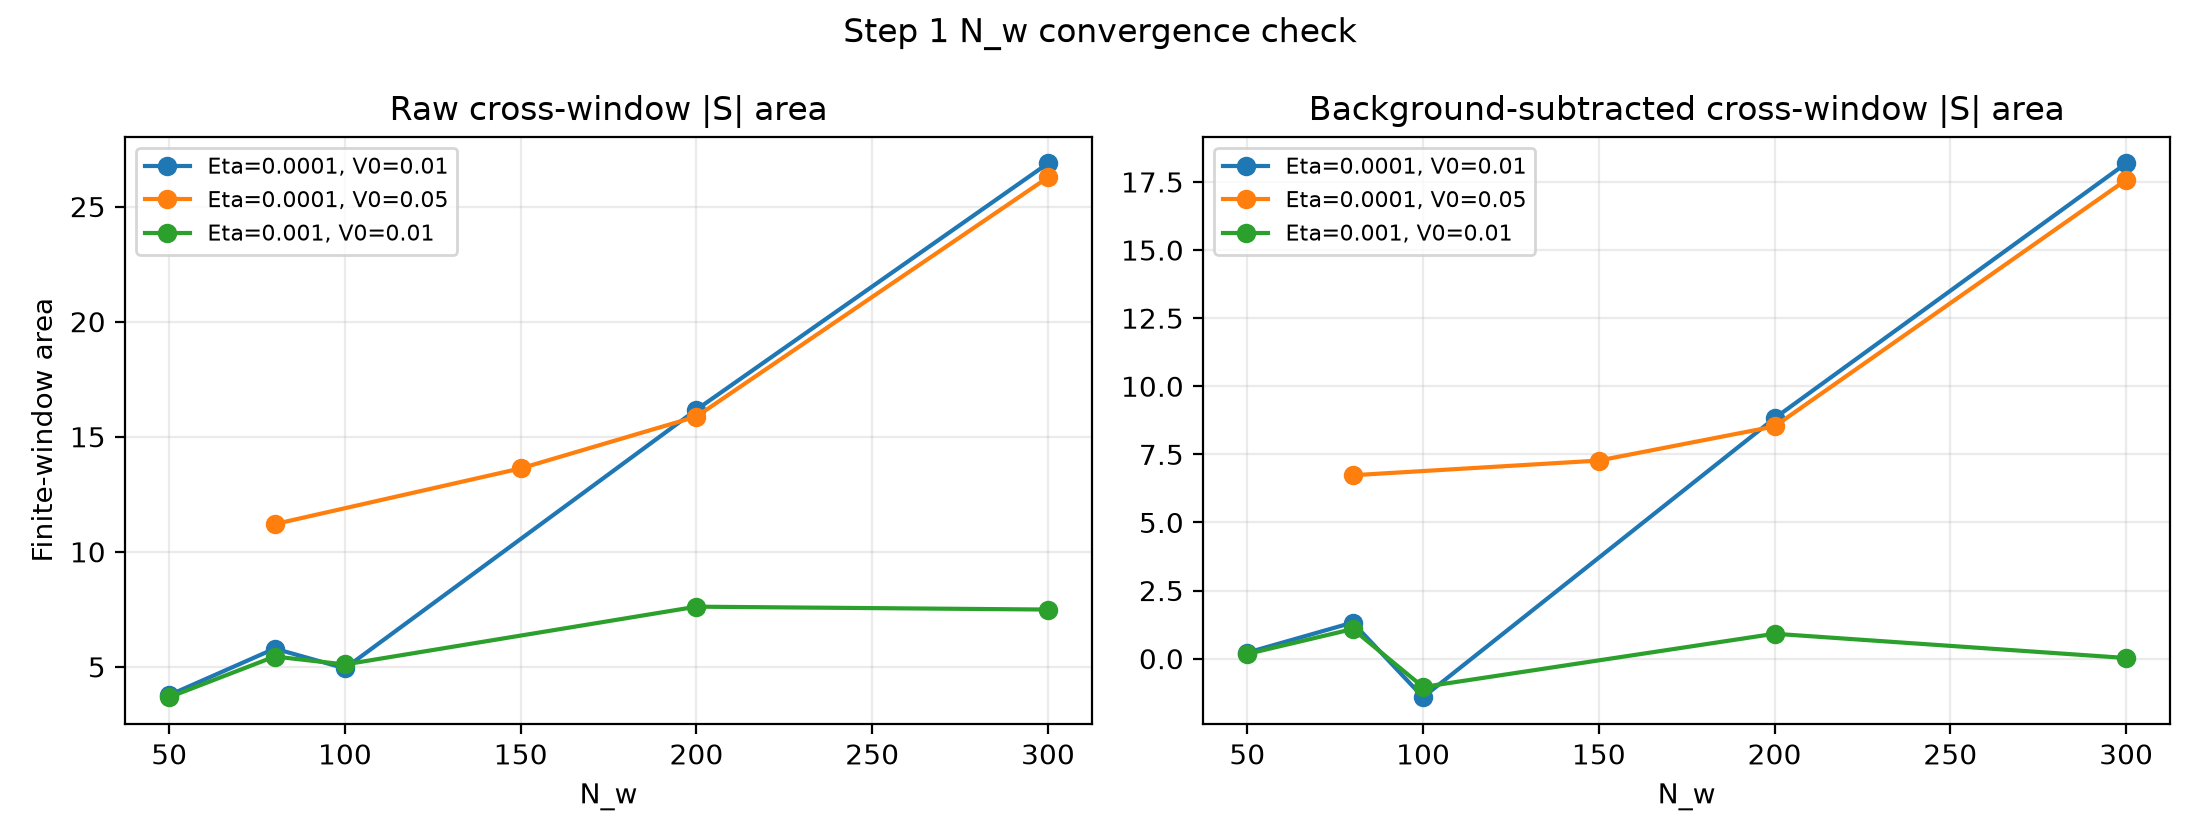
\includegraphics[width=\columnwidth]{nw_cross_abs_area_convergence.png}
\caption{
Step 1 convergence diagnostic.  The cross-window finite integral depends on
both linewidth and grid density.  The model response is present, but later
comparisons should be interpreted as controlled relative tests rather than as
fully converged absolute intensities.
}
\label{fig:step1}
\end{figure}

\section{Step 2: scalar separation of SOC, dimerisation, and spin correlations}

The second step tested whether three scalar contributions to bright--dark
mixing could be distinguished spectroscopically:
\begin{equation}
V_{BD}^{\mathrm{eff}}
= V_0+\lambda_\delta\delta+\lambda_C C_1 .
\end{equation}
Here $\delta$ is the spin-Peierls/dimerisation order parameter, while
$C_1=\langle \mathbf{S}_i\cdot\mathbf{S}_{i+1}\rangle$ is a local spin
correlation proxy.  The distinction is physical: $\delta$ vanishes above the
spin-Peierls transition, whereas $C_1$ can remain finite in the uniform chain.

Three cases were compared: constant SOC-like mixing, dimerisation-enhanced
mixing, and spin-correlation-enhanced mixing.  The dimerisation and
spin-correlation cases were matched to the same
$V_{BD}^{\mathrm{eff}}=0.02$, while the constant control used
$V_{BD}^{\mathrm{eff}}=0.01$.

\begin{table}[b]
\centering
\caption{Step 2 finite-window metrics for the rephasing component.}
\small
\begin{tabular}{lccc}
\toprule
Case & $V_{BD}^{\mathrm{eff}}$ & $A_{\mathrm{cross}}$ & diff. \\
\midrule
Constant & 0.01 & 10.210040 & -- \\
Dimer. & 0.02 & 13.682378 & $0.657$ \\
$C_1$ & 0.02 & 13.682378 & $2.62\times10^{-17}$ \\
\bottomrule
\end{tabular}
\label{tab:step2}
\end{table}

The result is decisive: the scalar model distinguishes weak and enhanced
effective mixing, but it cannot identify the microscopic origin of the
enhancement.  Dimerisation and $C_1$ produce numerically identical spectra when
they enter only through the same scalar $V_{BD}^{\mathrm{eff}}$.

\section{Step 3: dynamic lattice coordinate}

Step 3 added a truncated harmonic coordinate representing a dynamical lattice
degree of freedom.  The mixing Hamiltonian became
\begin{equation}
H_{\mathrm{mix}} =
V_{BD}^{\mathrm{static}} L_{BD}
+ g_Q Q L_{BD},
\end{equation}
with
\begin{equation}
Q=a+a^\dagger,
\qquad
V_{BD}^{\mathrm{static}}=
V_0+\lambda_\delta\delta+\lambda_C C_1 .
\end{equation}
The central question was whether adding the operator-valued term
$g_Q QL_{BD}$ creates spectral information that cannot be reproduced by a
static scalar $C_1$ control.

The two static controls remained identical at matched
$V_{BD}^{\mathrm{static}}=0.02$, reproducing the Step 2 degeneracy inside the
larger Hilbert space.  The dynamic dimerisation/phonon case, however, differed
strongly from the static controls.  The relative maximum full-spectrum
difference between dynamic and static dimerisation was $5.46\times10^{-1}$.

\begin{table}[t]
\centering
\caption{Step 3 rephasing finite-window metrics.}
\small
\begin{tabular}{lccc}
\toprule
Case & $g_Q$ & $A_{\mathrm{cross}}$ & cross/diag \\
\midrule
Static $C_1$ & 0 & 14.160315 & 0.142697 \\
Static $\delta$ & 0 & 14.160315 & 0.142697 \\
Dynamic $\delta$ & 0.010 & 11.761513 & 0.149235 \\
\bottomrule
\end{tabular}
\label{tab:step3}
\end{table}

\begin{figure}[t]
\centering
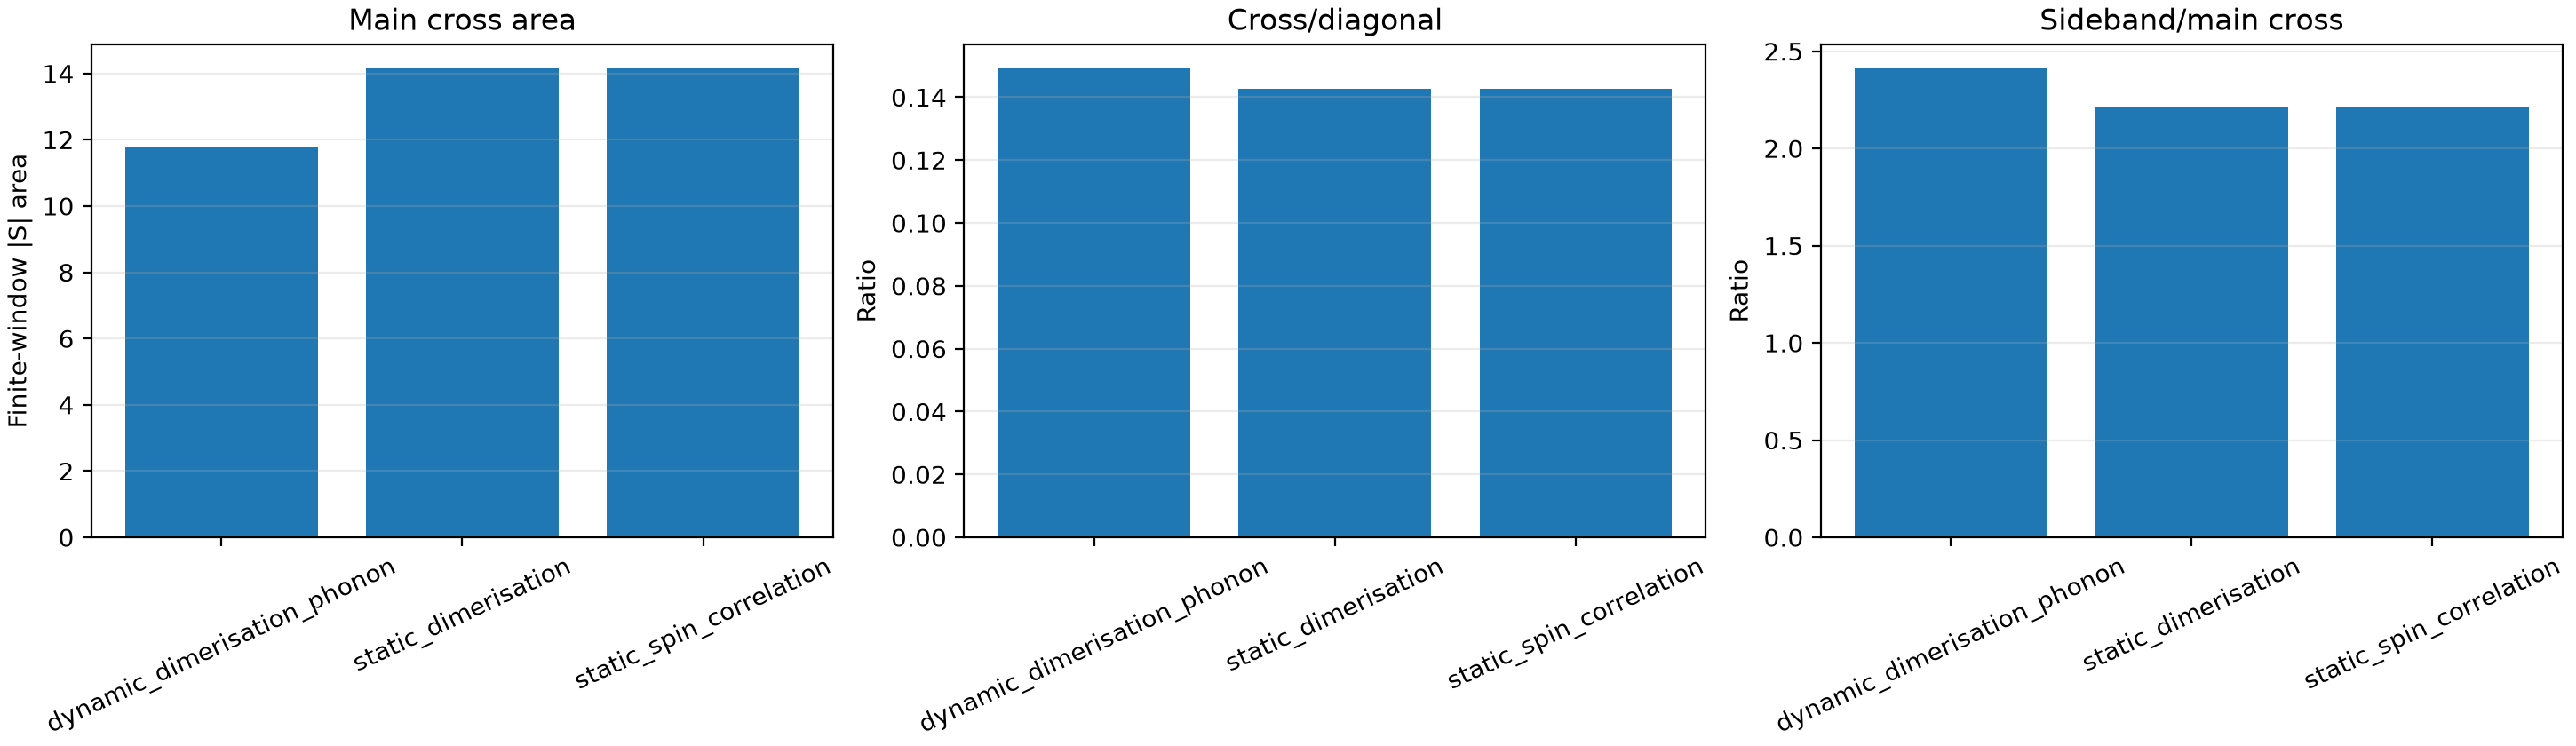
\includegraphics[width=\columnwidth]{step3_window_metrics.png}
\caption{
Step 3 aggregate metrics.  The static dimerisation and static spin-correlation
controls remain degenerate, while the dynamic phonon coordinate changes the
finite-window response and sideband-related metrics.
}
\label{fig:step3}
\end{figure}

The conclusion is that a lattice contribution must enter through a dynamical or
sector-specific degree of freedom if it is to be distinguishable from a scalar
local spin-correlation control.

\section{Step 4: independent temperature and field trends}

The fourth step introduced independent phenomenological trends for
dimerisation and local spin correlations.  The spin-Peierls transition
temperature was modeled as
\begin{equation}
T_{\mathrm{SP}}(B)
=\max\left[0,T_{\mathrm{SP},0}(1-\alpha_B B^2)\right],
\end{equation}
with
\begin{equation}
\delta(T,B)=
\begin{cases}
\delta_0\left(1-T/T_{\mathrm{SP}}(B)\right)^\beta,
& T<T_{\mathrm{SP}}(B),\\
0, & T\ge T_{\mathrm{SP}}(B).
\end{cases}
\end{equation}
The dynamic lattice coupling was scaled as
\begin{equation}
g_Q^{\mathrm{eff}} =
g_{Q0}\frac{\delta(T,B)}{\delta(T_{\mathrm{ref}},B_{\mathrm{ref}})}.
\end{equation}
In contrast, $C_1(T,B)$ was kept finite in both the dimerised and uniform
regimes.  This is the essential trend-level control: if $C_1$ were forced to
zero with $\delta$, one could not distinguish a spin-Peierls order parameter
from a generic spin-correlation channel.

\begin{table}[b]
\centering
\caption{Step 4 trend-level controls.}
\scriptsize
\begin{tabular}{lcccc}
\toprule
Case & $\delta$ & $C_1$ & $g_Q^{\mathrm{eff}}$ & $A_{\mathrm{cross}}$ \\
\midrule
Low-$T$ lat. & 0.007071 & -0.378667 & 0.010 & 12.554241 \\
High-$T$ off & 0 & -0.329471 & 0 & 10.919127 \\
High-$B$ off & 0 & -0.346199 & 0 & 10.919127 \\
High-$T$ $C_1$ & 0 & -0.329471 & 0 & 16.266623 \\
\bottomrule
\end{tabular}
\label{tab:step4}
\end{table}

\begin{figure}[t]
\centering
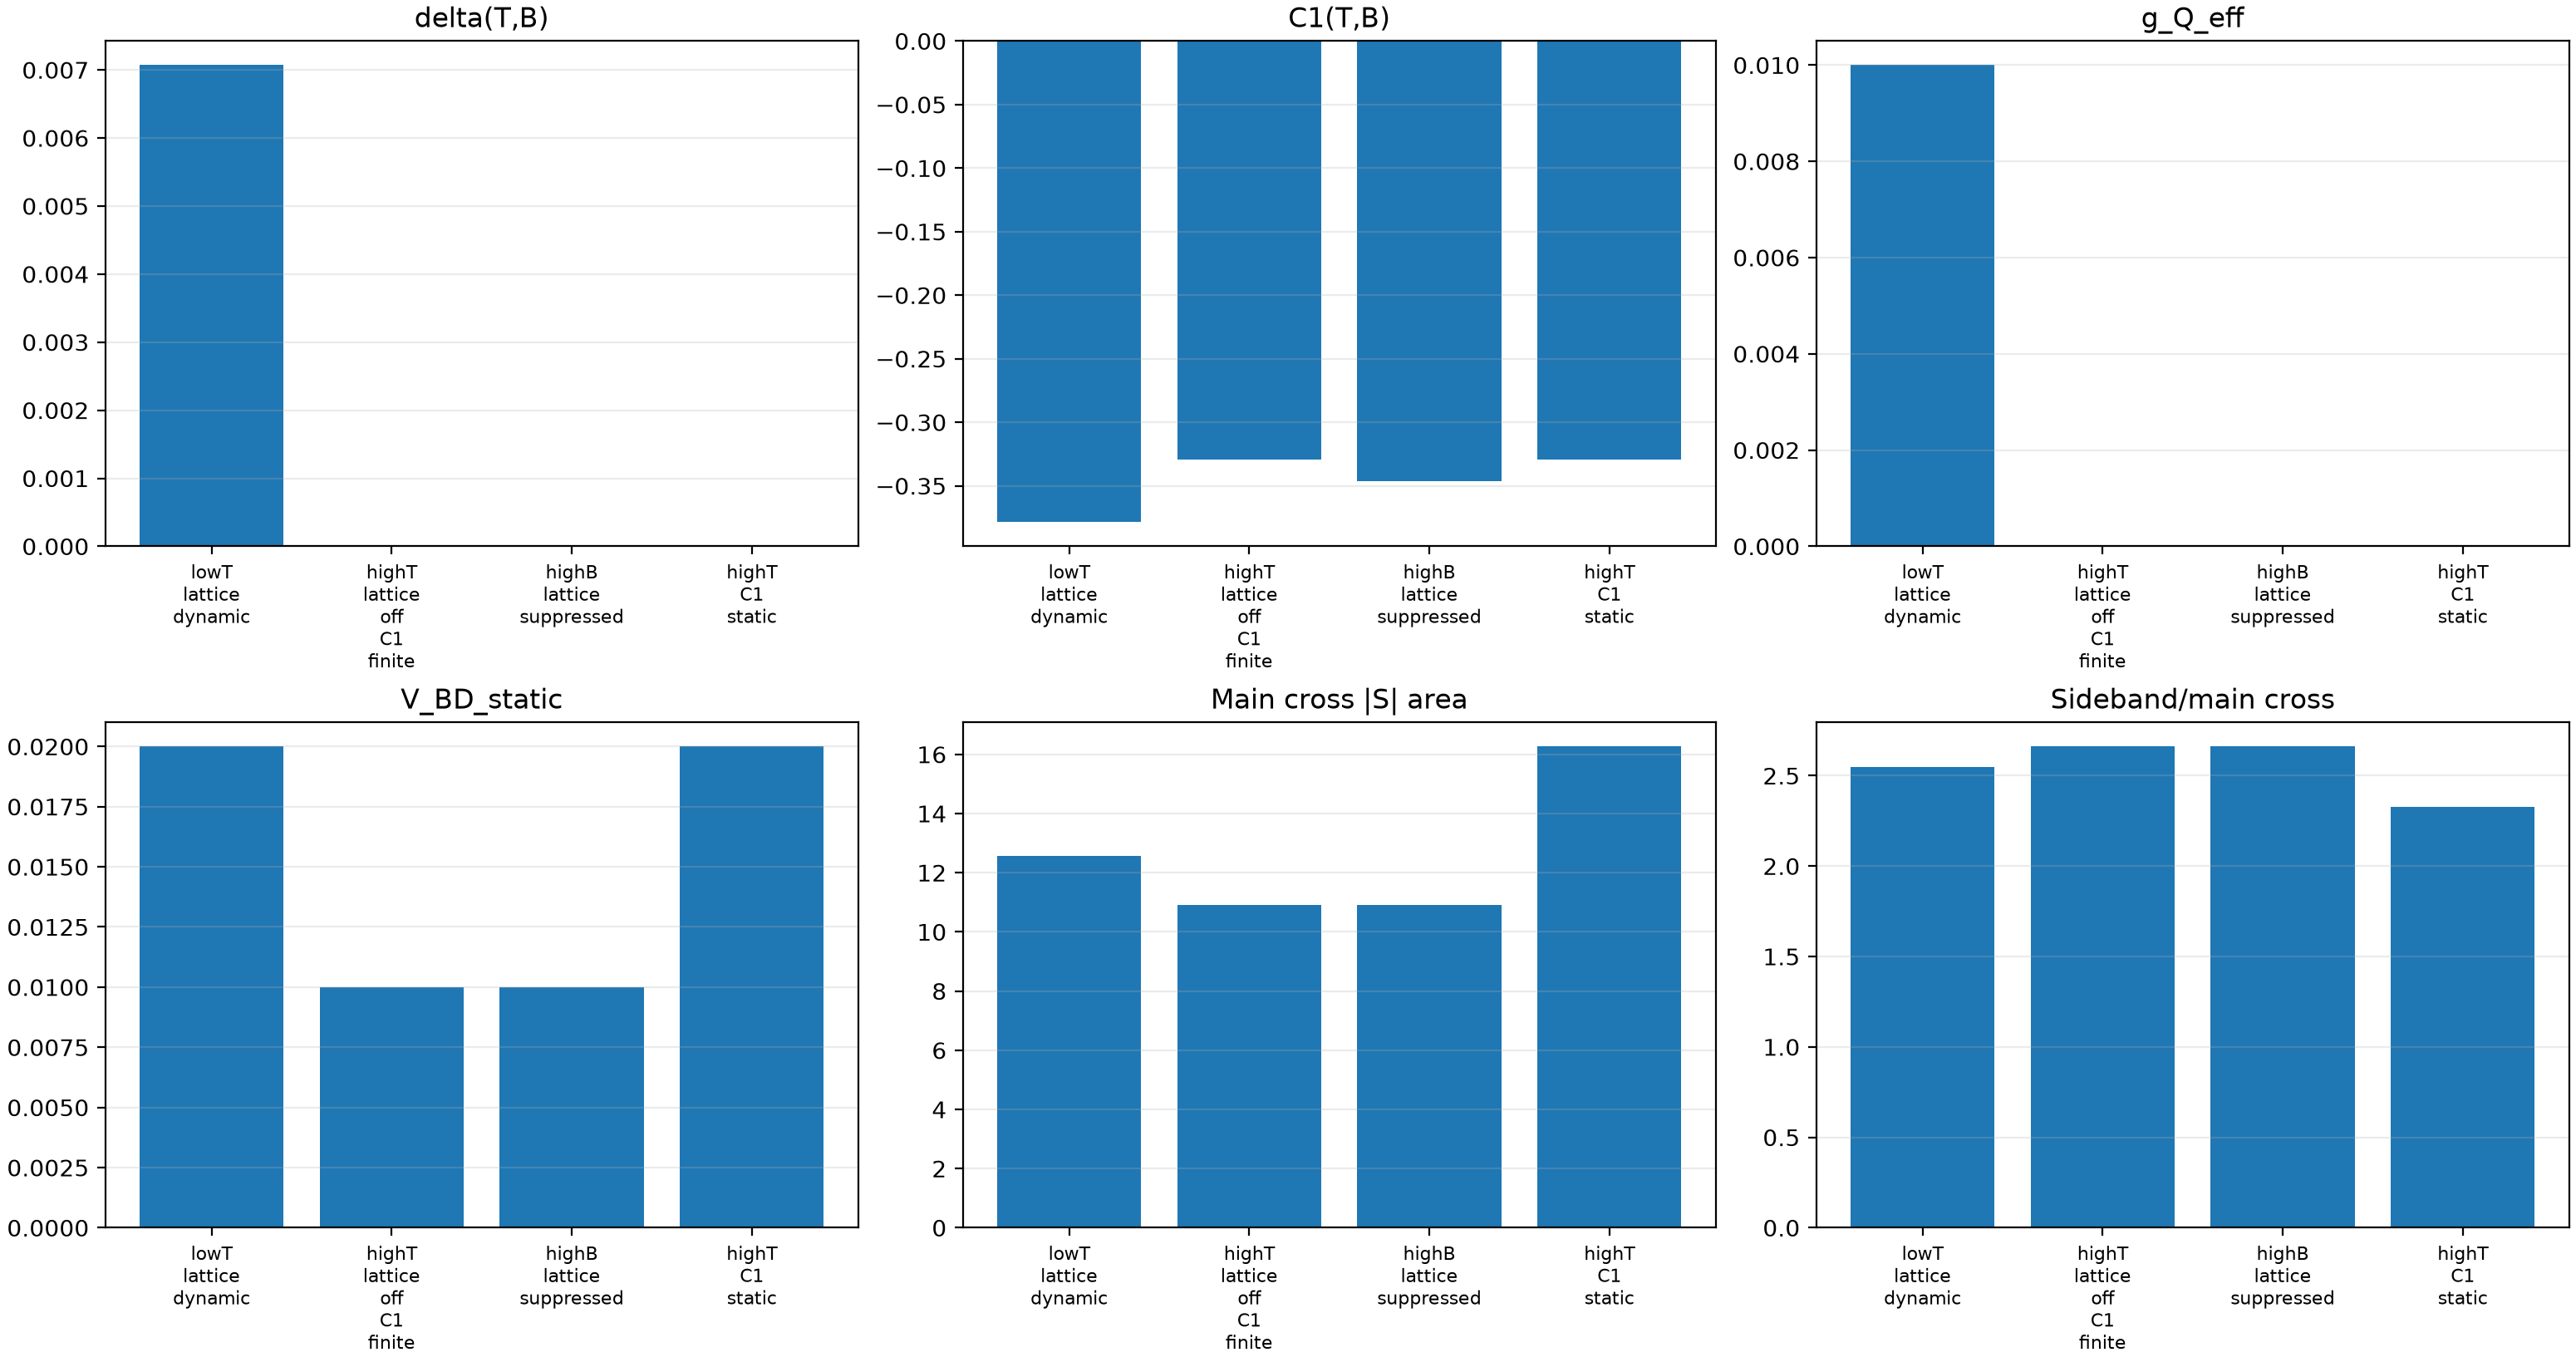
\includegraphics[width=\columnwidth]{step4_trend_metrics.png}
\caption{
Step 4 trend metrics.  The lattice channel follows $\delta(T,B)$ and turns off
above the transition or under field suppression, while the $C_1$-static control
can remain strong even when $\delta=0$.
}
\label{fig:step4}
\end{figure}

The low-temperature lattice case differs strongly from the high-temperature
lattice-off control, with relative maximum full-spectrum difference
$6.76\times10^{-1}$.  The high-field and high-temperature lattice-off controls
are identical in the minimal Hamiltonian because both have $\delta=0$,
$g_Q^{\mathrm{eff}}=0$, and the same scalar mixing.  The high-temperature
$C_1$ static control remains large even with $\delta=0$; its difference from
the high-temperature lattice-off baseline is $5.98\times10^{-1}$.

\section{Current interpretation}

The completed tests support four working conclusions.

First, the minimal bright--dark model is adequate as a numerical validation
platform.  It produces controlled diagonal and cross-peak responses, but
absolute finite-window intensities should be treated carefully because they
depend on linewidth and grid density.

Second, a scalar effective mixing
$V_{BD}^{\mathrm{eff}}=V_0+\lambda_\delta\delta+\lambda_C C_1$ is not enough
to identify whether an enhanced signal is caused by spin-Peierls dimerisation
or by local spin correlations.  At matched scalar mixing, the spectra are
identical.

Third, an explicit dynamical lattice coordinate provides a viable way to break
that degeneracy.  The operator-valued term $g_QQL_{BD}$ changes the nonlinear
response even when the static bright--dark mixing is held fixed.

Fourth, the correct experimental or phenomenological diagnostic should be
trend-based.  A feature that follows $\delta(T,B)$ and vanishes above the
spin-Peierls transition is compatible with lattice/spin-Peierls control.  A
feature that persists when $\delta=0$ but $C_1$ remains finite cannot be
assigned uniquely to the dimerised phase.

\section{Limitations and next steps}

The present model is intentionally minimal.  It does not yet include a true
spinon continuum, a rigorous momentum-sector treatment, or a microscopic
phonon bath.  Momentum integration has been kept off in the validated trend
tests in order to isolate the bright--dark and lattice controls.  This is a
reasonable staging choice, but it means that any comparison to a uniform
spin-chain regime remains phenomenological.

The next useful calculations are:
\begin{enumerate}
\item Sweep $T$ across $T_{\mathrm{SP}}$ and track the same finite-window
observables used in Step 4.
\item Sweep $B$ at fixed low temperature to test field suppression of the
lattice channel.
\item Scan $g_Q$ and $\omega_Q$ to identify which observables scale with the
dynamic phonon coordinate rather than with scalar mixing.
\item Only after the above controls are stable, revisit momentum-sector
coherence and possible spinon-inspired response functions.
\end{enumerate}

\section{Summary}

The main modeling lesson is that ``SOC sensitivity'' cannot be inferred from a
temperature-dependent nonlinear feature alone.  In a spin-Peierls material, a
low-temperature enhancement can arise from lattice dimerisation, from local
spin correlations, or from genuine SOC-enabled bright--dark mixing.  The tests
completed so far define a practical hierarchy of controls: validate the minimal
bright--dark response, show the failure of scalar separation, add a dynamic
lattice coordinate, and finally compare independent temperature/field trends.
This provides a concrete foundation for the next phase of the CuGeO$_3$
modeling effort without prematurely committing to a full microscopic spin-chain
solver.

\end{document}
